\chapter{Benchmark Results}    \label{sec:results}

In this section, we seek to determine the overhead that indirect addressing imposes on unstructured grids compared to regular grid runtimes, and assess the effectiveness of our optimized approaches. We do this by implementing three real-world stencils, called \emph{Laplace-of-Laplace (laplap)}, \emph{horizontal diffusion (hdiff)}, and \emph{fastwaves}, using our previously described methods for grid access and grid storage (see sections \ref{sec:optimizations} and \ref{sec:grid-implementations}). We use key profiler metrics to better understand what causes the differences in performance.

Real-world stencil applications are applied in a multitude of different scenarios: problem domain sizes, precision requirements and properties of the stencils vary. In combination with the various grid access and grid storage methods we described, this leaves a large number of combinations to be tested. In our benchmarks, we assessed the performance impact of the following properties:

\begin{itemize}
    \item 
        Input/output conditions 
        \begin{itemize}
            \item Domain size (size of the input and output grids)
            \item Required precision (single or double floating-point number precision)
        \end{itemize}
    \item
        Stencil properties, such as the \emph{depth and number of neighbor dependencies}, the \emph{number of input and output fields} (number of different values stored in a cell) and the \emph{arithmetic intensity}
    \item
        \emph{Kernel launch configuration:} number of threads, blocks, and bytes of shared memory
	\item Implementation of stencil, i.e. the used \emph{grid access scheme}
    \item
        Grid storage implementation properties
        \begin{itemize}
            \item Memory layout and potential regular patterns in grid structure
            \item 
                Memory layout of neighborship storage
                \begin{itemize}
                    \item Depth of stored neighbor pointers (pointer \emph{chasing} vs. \emph{non-chasing})
                    \item Compression of neighborship table
                \end{itemize}
        \end{itemize}

\end{itemize}

\section{Setup and Benchmarked Stencils}\label{sec:benchmark-setup}

The three benchmarked stencils represent real-world use cases in meteorology. Table \ref{tab:benchmarked-stencils} details the values of the main stencil characteristics (those listed in the second main bullet point above). Note the increasing complexity and number of fields required from the \emph{laplap} to the \emph{fastwaves} stencil. Also note that the \emph{fastwaves} stencil, otherwise the most complex, does not require access to neighbors-of-neighbors.

\begin{table}
	\makebox[\textwidth][c]{                                     
		\begin{tabular}{m{4cm} m{1.25cm} m{1.25cm} m{1.25cm} m{1.25cm} m{4cm}}
		    \textbf{Stencil}  &  \multicolumn{3}{c}{\textbf{Neighborhood}}  &  \textbf{Fields}  &  \textbf{Arithmetic Intensity} \\
		    \cline{2-4}
		    &  \textbf{X}  &  \textbf{Y}  &  \textbf{Z}  & \\
		    \hline
			\hline
		    \raggedright Laplace-of-Laplace \emph{(laplap)}  &  (-2, 2)  &  (-2, 2)  &  0  &  1  & {\raggedright Add., Mult., Sub.} \\
			\hline
		    \raggedright Horizontal Diffusion \emph{(hdiff)}  &  (-2, 2)  &  (-2, 2)  &  0  &  2  &  {\raggedright Add., Mult., Sub., Branches} \\
			\hline
		    \raggedright \emph{Fastwaves}  &  (0, 1)  &  (0, 1)  &  (-1, 1)  &  9  & {\raggedright Add., Mult., Sub., Div., Branches} \\
		    \hline
		\end{tabular}
	}
	\caption{\label{tab:benchmarked-stencils}Stencil characteristics. The neighborhood is given as an interval around the coordinates of a cell, i.e. $(-2, 2)$ means neighbors-of-neighbors are required for the stencil output calculation. The stencils are listed by their regular grid runtime in ascending order. Note that the \emph{fastwaves} stencil is the only stencil with dependencies in the Z-dimension, has the highest arithmetic intensity, and accesses the biggest number of fields.}
\end{table}

The calculations performed by the stencils are defined in terms of a regular grid. All three stencils require neighborships as in regular grids (top, left, bottom, right, front, back). To measure the cost of using an unstructured grid, we represent the same regular grid in an unstructured fashion, using two memory layouts, \emph{row-major} and \emph{z-order-curves} (see section \ref{sec:emulating}). This can be thought of as \emph{emulating} an unstructured grid. Even if the grid structure is entirely regular, we store and access it in the same fashion as we would for a truly unstructured grid in the unstructured benchmarks. Retaining regularity even in the unstructured representation is required to maintain comparability of the results of the unstructured variants with the regular variants. We note that this approach to benchmarking might fail to capture some effects of real unstructured grids with actual irregularities.

For all stencils, we created several variants; for each of the grid access optimizations described in section \ref{sec:optimizations} we implemented a separate CUDA kernel. During the implementation process, the results of each of those variants are verified against an unoptimized reference implementation of the stencil running on the CPU to assure the correctness of the results. In all variants, the implementation of the actual output calculations (as per stencil definition) remains completely unchanged. Only the portions of code responsible for index calculations/lookups (for neighborship access) are swapped out. This is achieved by using \emph{C preprocessor macro definitions} in all places where indexing or neighborship access is required. The macro definitions are then redefined in each variant to either use direct or indirect addressing for the regular and unstructured grids, respectively (with further variations for non-chasing/chasing and compressed/uncompressed neighborship tables).

The stencils were benchmarked on an \emph{Nvidia Tesla V100} GPU. This GPU implements the \emph{Volta} architecture by Nvidia with compute capability $7.0$. The reported run times are the median of 20 timed kernel runs. Before the first one of the timed kernel runs, an untimed \emph{warm-up run} is performed (see the last paragraph section \ref{sec:arguing} for the reasoning behind this). The GPU is reset using an API call to \texttt{cudaDeviceReset()} between each run to flush caches and to free device memory from previous runs. The grid values and neighborship relations (for unstructured grids) are stored in unified global memory and are pre-transferred to the GPU and back to the host (\texttt{cudaMemPrefetchAsync()}) before respectively after the kernels are run. Memory transfer from host to device and back is, therefore, \emph{not} part of the reported run times.

\section{Overview of Results}

\begin{figure}
    % >>> fas=u.groupmin(df[(df["size-z"]==64)&df["z-curves"]], by=u.col.problem+u.col.access+u.col.storage)
    % >>> fas=u.add_colors_markers(fas, color="variant")
    % >>> reg=u.groupmin(df[(df["size-z"]==64)&~df["unstructured"]], by=u.col.problem)
    % >>> reg["variant"]="regular"
    % >>> reg["color"]="black"
    % >>> x=pd.concat([fas,reg])
    % >>> u.barplot(x[x["stencil"]=="fastwaves"], grp=u.col.storage+["unstructured"], cat=u.col.access, cat_pretty=["variant"], grp_pretty=["no-chase", "comp"])
    % <matplotlib.axes._subplots.AxesSubplot object at 0x124582ed0>
    % >>> plt.ylabel("Median runtime [μs]")
    % Text(0, 0.5, 'Median runtime [μs]')
    % >>> fig=u.plotdone(legend=2)
    % >>> fig.set_size_inches(6,3)
    % >>> u.plotsave("report/img/overview-fastwaves.pdf", fig)
	\begin{center}
	    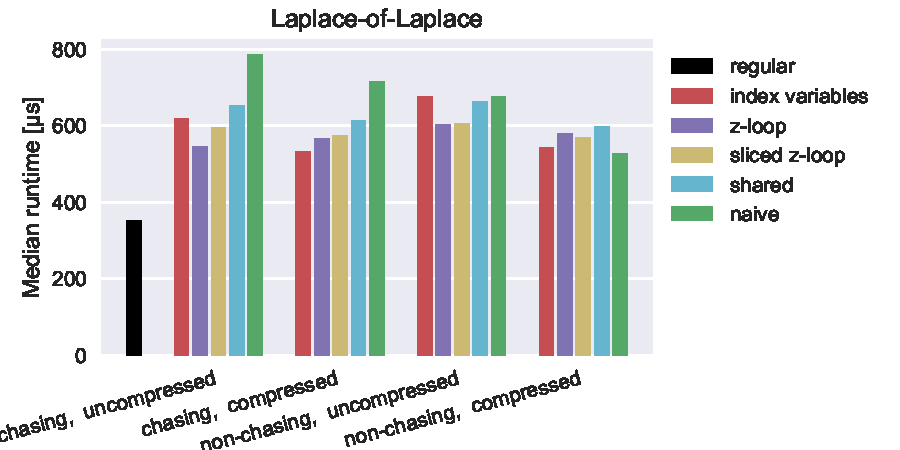
\includegraphics[scale=0.75]{overview-laplap.pdf}
    
	    \vspace{0.5cm}
    
	    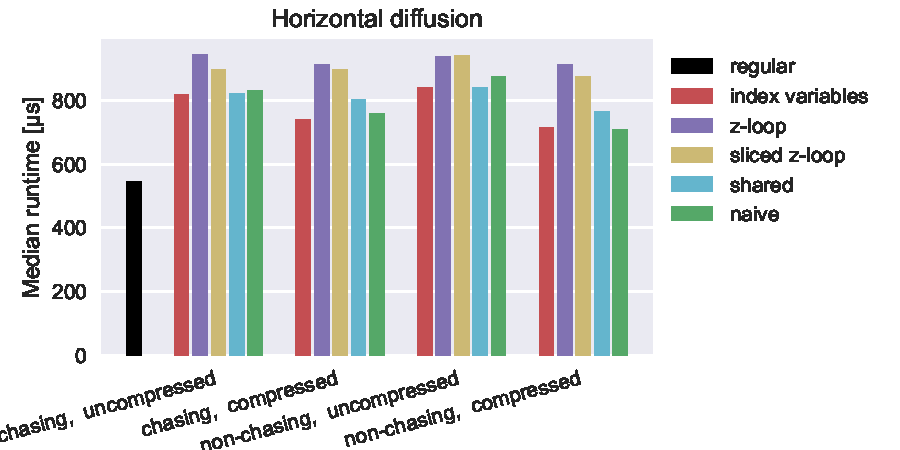
\includegraphics[scale=0.75]{overview-hdiff.pdf}
    
	    \vspace{0.5cm}
    
	    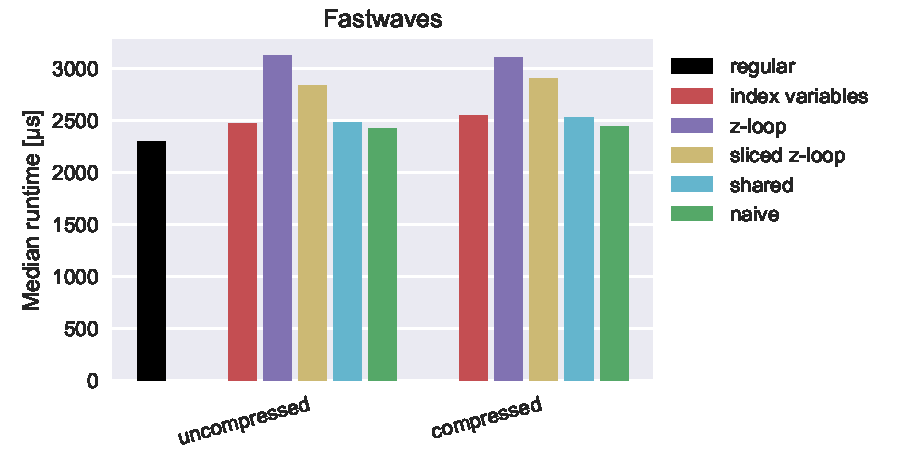
\includegraphics[scale=0.75]{overview-fastwaves.pdf}
		
    \end{center}
    \caption{\label{fig:storage-access} Overview of runtimes for all tested stencil implementations. The various grid access strategies implemented are represented as categories (colors of the bars), while the used data structures for the neighborship table (grid storage strategy) are shown as groups of bars on the X-axis. We report the median value across 20 runs, using the fastest respective launch configuration for each bar. The grid size is $512\times 512\times 64$ and the \emph{z-curves} memory layout is used for the unstructured grids in this example. The input and output values are double-precision floating-point numbers.}
\end{figure}

\begin{table}
	\begin{center}
    \begin{tabular}{l c c l c r} % c c}        
        \multicolumn{6}{c}{\textbf{Laplace-of-Laplace Stencil}} \\
        \hline
        \hline
        %& & & & \multicolumn{2}{c}{$512\times 512\times 64$ Grid} & \multicolumn{2}{c}{$128\times 128\times 64$ Grid} \\
        %\cline{5-6} %\cline{7-8} 
        Storage & (1) & (2) & Access Strategy  & Runtime & Slowdown \\ %& Runtime & Slowdown \\
        \hline 
        \multicolumn{3}{l}{regular grid baseline} & index variables & $353 \mu s$ & -\\
        \hline
         row-major & \checkmark & \checkmark & index variables &  $\mathbf{512 \mu s}$ & $\mathbf{45 \%}$ \\
         row-major & - & \checkmark & index variables & $515 \mu s$ & $46 \%$ \\
         row-major & \checkmark & - & sliced z-loop & $582 \mu s$ & $65\%$ \\
         row-major & - & - & sliced z-loop & $608 \mu s$ & $72 \%$ \\
        \hline
         z-curves & - & \checkmark & naive & $\mathbf{528 \mu s}$ & $\mathbf{50 \%}$ \\
         z-curves & \checkmark & \checkmark & index variables & $532 \mu s$ & $51 \%$ \\
         z-curves & \checkmark & - &  z-loop & $546\mu s$ & $55 \%$ \\
         z-curves & - & - & z-loop & $603 \mu s$ & $71 \%$ \\
        
        \hline
        \hline \\
        \multicolumn{6}{c}{\textbf{Horizontal Diffusion Stencil}} \\
        \hline
        \hline
        Storage & (1) & (2) & Access Strategy  & Runtime & Slowdown \\
        \hline
        \multicolumn{3}{l}{regular grid baseline} & index variables & $546 \mu s$ & - \\
        \hline
          row-major & - & \checkmark & naive & $\mathbf{683 \mu s}$ & $\mathbf{25 \%}$ \\
        
         row-major & \checkmark & \checkmark & index variables & $731 \mu s$ & $34 \%$ \\
        
         row-major & \checkmark & - & index variables & $804\mu s$ & $47\%$ \\
         &   & &  shared (tie) & $804\mu s$ & $47\%$ \\
         row-major & - & - & naive & $845 \mu s$ & $55 \%$ \\
        \hline
         z-curves & - & \checkmark & naive & $\mathbf{710 \mu s}$ & $\mathbf{30 \%}$ \\
         z-curves & \checkmark & \checkmark & index variables & $741 \mu s$ & $36 \%$ \\
         z-curves & \checkmark & - & index variables & $820\mu s$ &  $50 \%$ \\
         z-curves & - & - & shared & $841 \mu s$ & $54 \%$ \\
        
        \hline
        \hline\\
        \multicolumn{6}{c}{\textbf{Fastwaves Stencil}}\\
        \hline
        \hline
        Storage & (1) & (2) & Access Strategy  & Runtime & Slowdown \\
        \hline
        \multicolumn{3}{l}{regular grid baseline} & naive & $2298 \mu s$ & - \\
        \hline
        row-major & & - & naive & $\mathbf{2400\mu s}$ & $\mathbf{4.4 \%}$ \\
        row-major & & \checkmark & naive & $2433\mu s$ & $5.9 \%$ \\
        \hline
        z-curves & & - & naive & $\mathbf{2426\mu s}$ & $\mathbf{5.6 \%}$ \\
        z-curves & & \checkmark & naive & $2438\mu s$ & $6.1 \%$ \\
        \hline\hline
    \end{tabular}
	\end{center}
    \begin{enumerate}[label=(\arabic*)]
        \item \textbf{Pointer Chasing?} (A checkmark means that only directly adjacent neighbors are stored and pointer chasing occurs for neighbor-of-neighbor access. No checkmark means neighbors-of-neighbors are explicitly stored in the neighborship tables.)
        \item \textbf{Compressed?} (A checkmark means the neighborship table was compressed by having all cells with identical relative neighbor offsets share their entries. This requires an additional lookup.)
    \end{enumerate}
    \caption{\label{tab:overview} Fastest access strategy for all grid storage options. \emph{Z-curves} and \emph{row-major} refer to the memory layout of the \emph{values} of the grid, whereas \emph{chasing/non-chasing} and \emph{compressed/uncompressed} are properties of the neighborship table. The runtimes are the median of 20 runs using the fastest respective launch configuration per benchmark. The slowdown is relative to the fastest regular grid implementation. The stencils were executed on a $512\times 512\times 64$-sized grid of double-precision floating-point numbers.}
\end{table}

Overall, we observed slowdowns around $1.5x$, $1.3x$ and $1.05x$ compared to fastest regular grid performance for the \emph{laplap}, \emph{hdiff} and \emph{fastwaves} stencils, respectively. Figure \ref{fig:storage-access} shows an overview of the overhead for all tested combinations of storage and access strategy on a large grid of size $512\times 512\times 64$. Table \ref{tab:overview} lists the fastest access strategy, the runtimes and the overheads for the three stencils in all possible storage configurations. For different domain sizes, see section \ref{sec:res-size}. We chose to display the results for a \emph{z-curve} layout, but results for the \emph{row-major} benchmarks are similar. The fastest launch configuration is plotted for each bar; for a more detailed analysis of what block sizes are beneficial to the different access strategies, see section \ref{sec:res-blocksize}. A more in-depth analysis of the different storage and access strategies is given in sections \ref{sec:res-storage} and \ref{sec:res-access} respectively.